\documentclass{handout}

% \SetInstructor{Lt Col James Phillips}
\SetCourseTitle{ECE231: Electrical Circuits and Systems I}
\SetSemester{Fall 2016}
\SetHandoutTitle{Lecture 29: Phasors Circuit Analysis and Design Part 1}

%\SetDueDate{1 Jan 2016}
%\ShowAllBlanks

\showsoln \setsolncolor{red}

\begin{document}
\maketitle

\textbf{OBJECTIVES:}
\begin{enumerate}
\item Learn to apply circuit analysis techniques we already know to solve circuits in the phasor domain
\end{enumerate}

\textbf{READING}
\begin{description}
\item [Required]:
Textbook, section 8.3, pages 391--402
\item [Optional]:
\end{description}

\section{Introduction}
Over the next couple of lessons we will be applying techniques we have already learned to phasor domain circuits.  The only thing that will be different is that we will be working with phasors (complex numbers) instead of real numbers.  If you can get over that hump this will feel like a lot of review.  We will look at:
\begin{enumerate}
\item Parallel and series combinations of \textbf{Impedances}
\item Voltage and Current Division
\item Mesh and Node Analyisis
\item Proportionality and Superposition
\item Thevenin and Norton equivalent circuits
\end{enumerate}

All these things still apply to phasor domain circuits. As a reminder, phasor analysis only applies to the steady state sinusoidal responses.  Phasor analysis does not tell you anything about the transient response.

\section{Resistance and Reactance}
In the way of some quick preliminaries we will introduce a new term, \textbf{reactance}.  We saw in last class that a phasor is just a complex number.  Any complex number can be written as $Z = R +jX$ where $R$ is the real part and $X$ is the imaginary part.  When we use complex numbers to represent impedances, $Z$, we call the real part, $R$, resistance and the imaginary part, $X$, the reactance.  $R$ is always positive, but $X$ can be positive or negative. A positive $X$ is called an {\em inductive} reactance, while a negative $X$ is a {\em capacitive} reactance.

\section{Series and Parallel Impedances}
Good News!  We have nothing new to learn here... Remember our derivation about how to add resistances?  It all started with KVL, KCL and Ohm's law.  Since all those laws apply to impedances, impedances add like resistance.

For series impedances:
\soln{1in}{
\[
Z_{eq} = Z_1+Z_2+Z_3+.....+Z_k =\sum_{n=1}^k Z_n
\]
}

For parallel impedances:
\soln{1in}{
\[
Z_{eq} = \frac{1}{\frac{1}{Z_1}+\frac{1}{Z_2}+\frac{1}{Z_3}+.....+\frac{1}{Z_k}} =\left[\sum_{n=1}^k \frac{1}{Z_n}\right]^{-1}
\]
}

\textbf{Example 1} -- For the circuit shown in Figure \ref{fig: Example1}, find $Z_{eq}$ given $\omega = 2000\ \frac{rad}{s}$

\begin{figure} [h!]
\centering
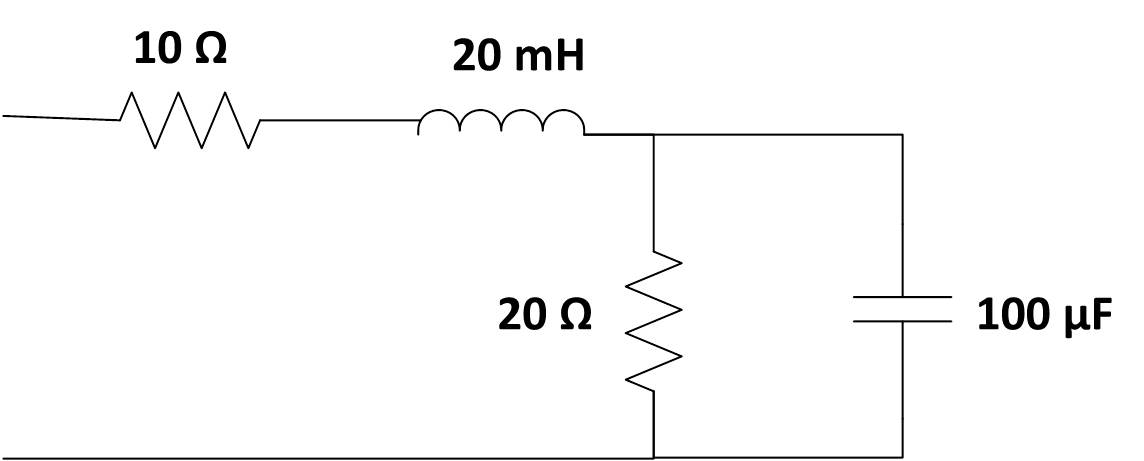
\includegraphics[width=0.7\textwidth]{Example1.jpg}
\caption{Circuit to accompany Example 1}
\label{fig: Example1}
\end{figure}

\soln{3in}{
\begin{figure} [h!]
\centering
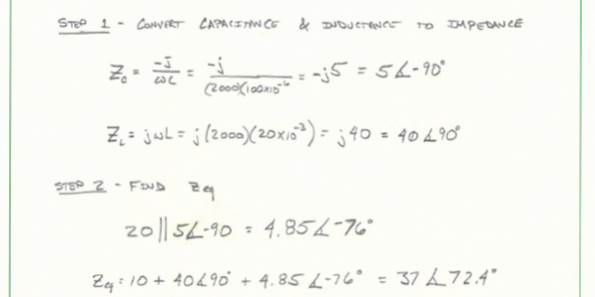
\includegraphics[width=1\textwidth]{Example1soln.jpg}
\end{figure}
}
\newpage
\clearpage
\pagebreak
\section{Voltage Division}
We will use some examples to show that voltage division also works with phasors.  Remember, voltage division applies to resistances (now impedances) in series.

\textbf{Example 2}-- For the circuits shown in Figures \ref{fig: Example2a} and \ref{fig: Example2b}, use voltage division to find the voltages across all resistors and the capacitor.

\begin{figure} [h!]
\centering
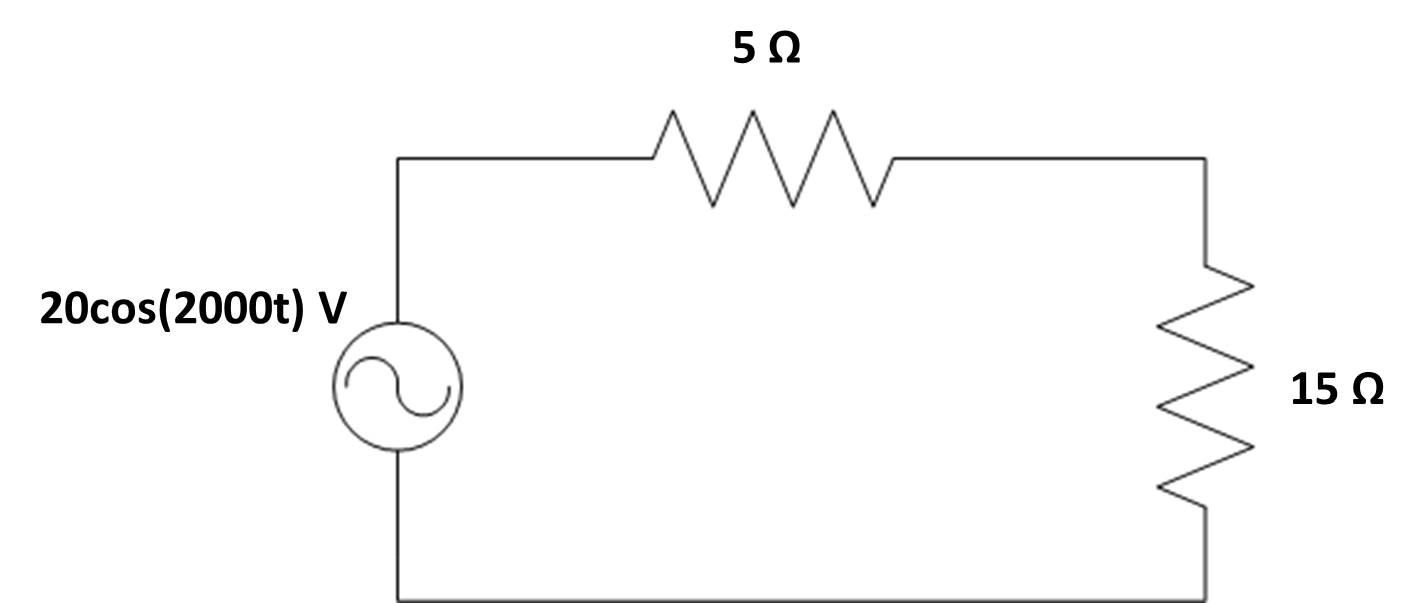
\includegraphics[width=0.7\textwidth]{Example2a.jpg}
\caption{Circuit to accompany example 2}
\label{fig: Example2a}
\end{figure}
\begin{figure} [h!]
\centering
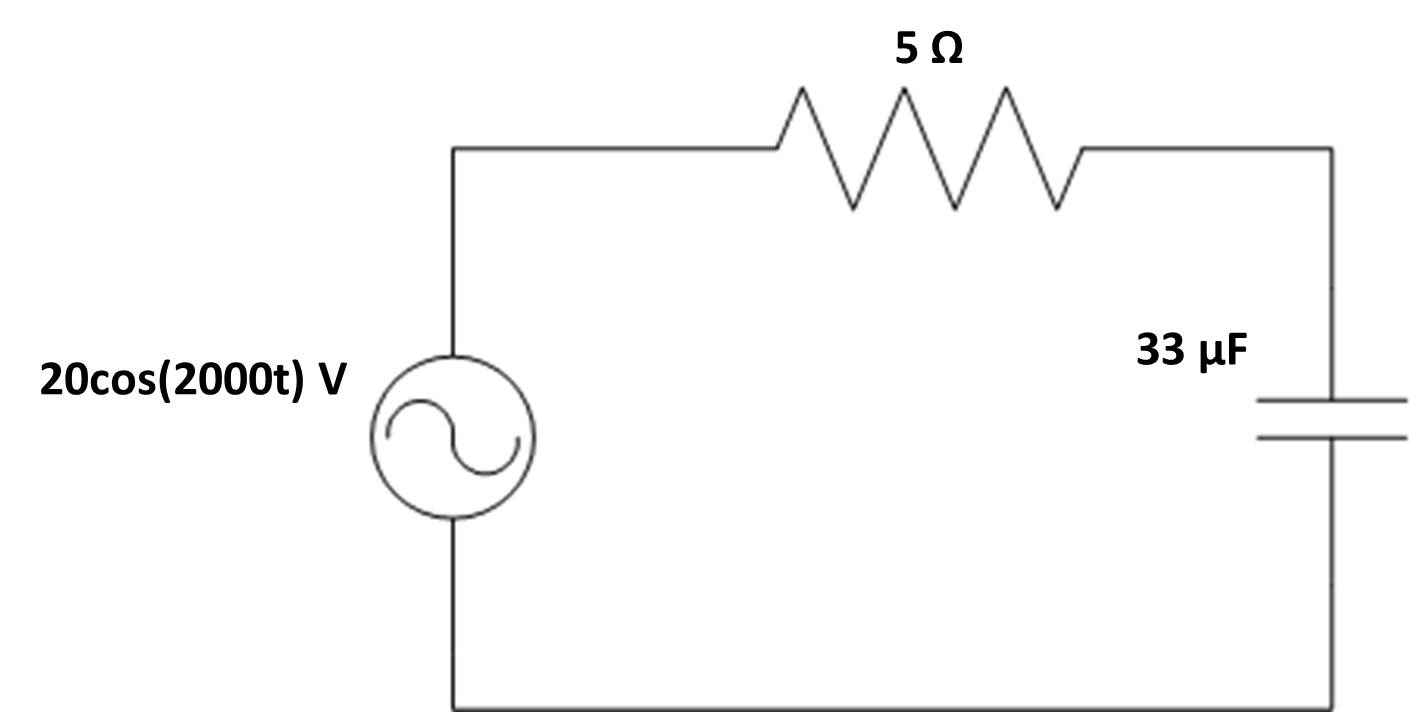
\includegraphics[width=0.7\textwidth]{Example2b.jpg}
\caption{Circuit to accompany example 2}
\label{fig: Example2b}
\end{figure}

\soln{3in}{
\begin{figure} [h!]
\centering
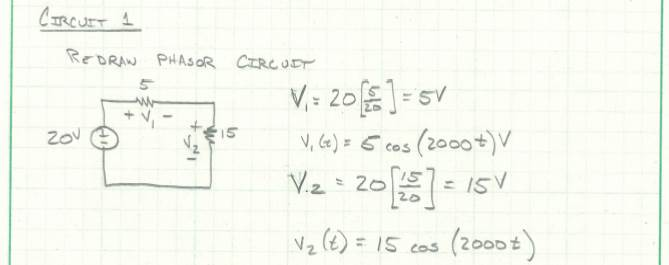
\includegraphics[width=1\textwidth]{Example2solnA.jpg}
\end{figure}
}
\soln{6in}{
\begin{figure} [h!]
\centering
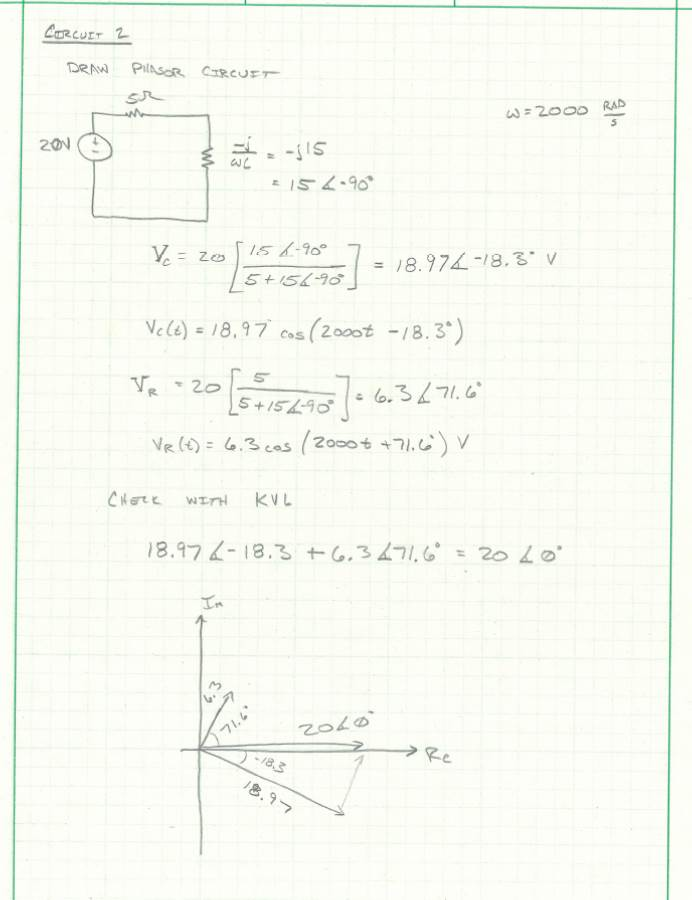
\includegraphics[width=1\textwidth]{Example2solnB.jpg}
\end{figure}
}

\newpage
\clearpage
\pagebreak

\section{Current Division}
Now we move onto some examples to show that current division also works with phasors.  Remember, current division applies to resistances (now impedances) in parallel.

\textbf{Example 3}-- For the circuit in Figure \ref{fig: Example3}, use current division to find the current through the inductor.
\begin{figure} [h!]
\centering
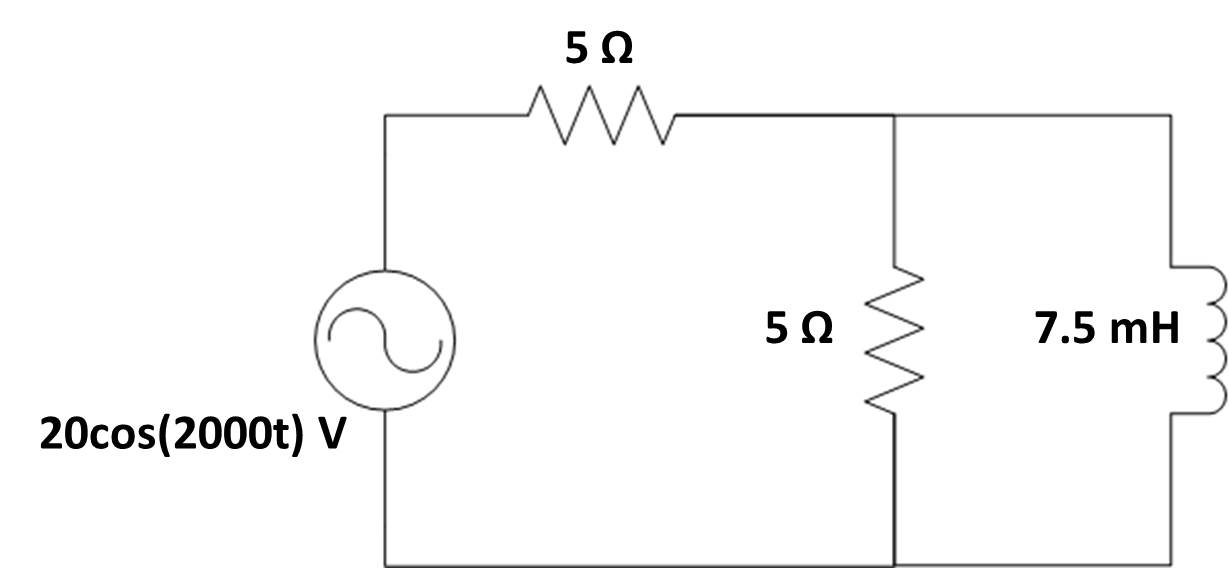
\includegraphics[width=0.5\textwidth]{Example3.jpg}
\caption{Circuit to accompany example 3}
\label{fig: Example3}
\end{figure}

\soln{6in}{
\begin{figure} [h!]
\centering
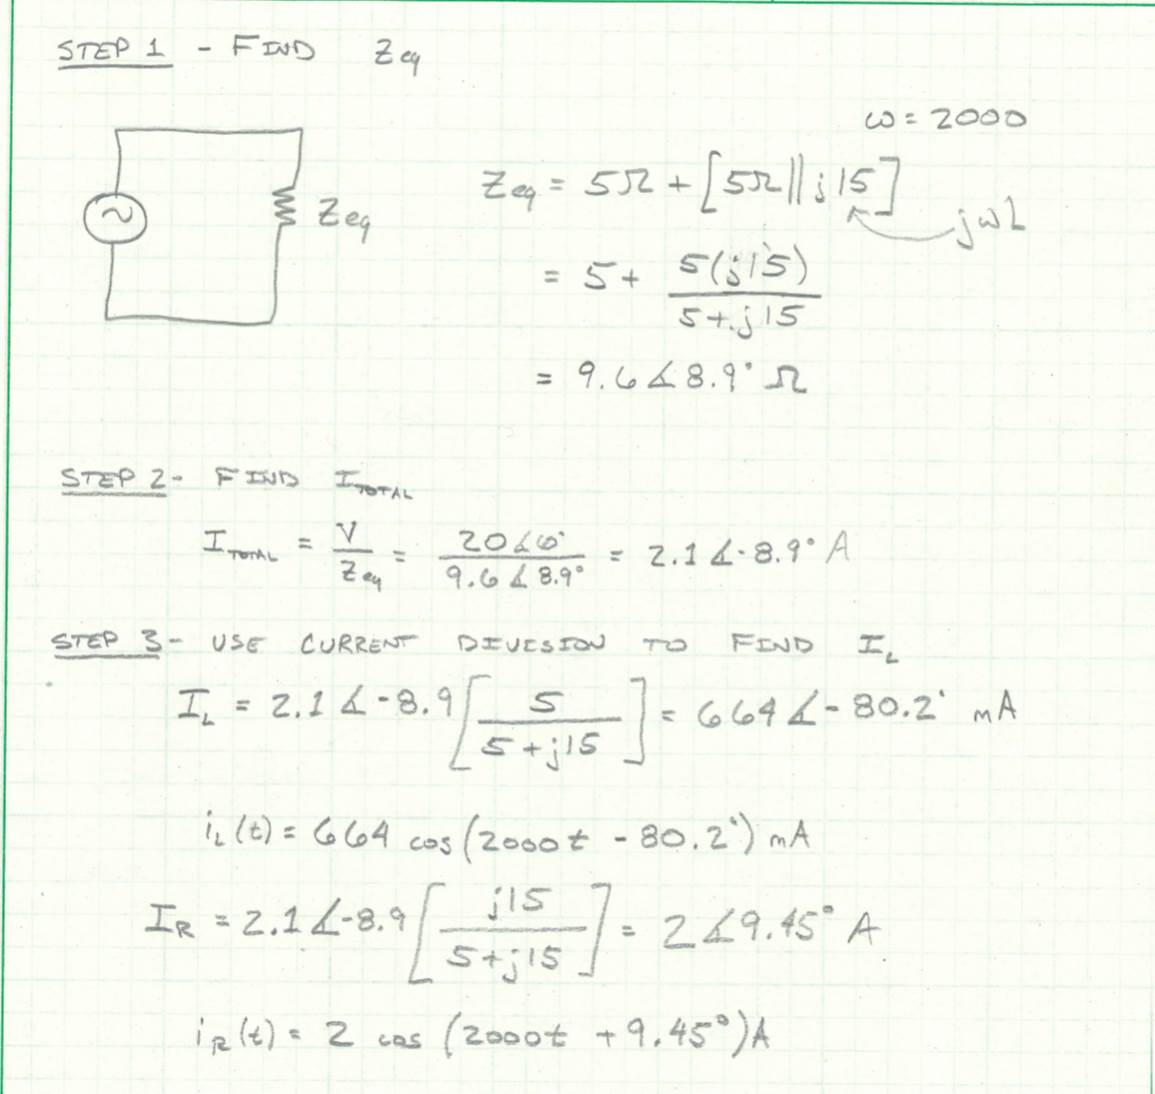
\includegraphics[width=0.9\textwidth]{Example3soln.jpg}
\end{figure}
}

\newpage
\clearpage
\pagebreak

\section{Mesh Analysis}
Recall the steps for mesh analysis:
\begin{enumerate}
\item Assign a current to each mesh
\item Assign a voltage (magnitude and polarity) to each device in the circuit
\item Write Kirchhoff's Voltage Law (KVL) equations for each mesh
\item Use device $i$--$v$ characateristics to rewrite KVL eqations from the previous step in terms of mesh currents
\item Rewrite equations in standard (matrix) form \& solve
\end{enumerate}

Also recall that the rules above specifically apply to circuits that do not contain any current sources.  We offered three techniques for dealing with current sources: source transformation, ensure the current source is only part of one mesh,  or use a supermesh.

\textbf{Example 4}-- Let's re-solve example 3 using Mesh Analysis.
\soln{6in}{
\begin{figure} [h!]
\centering
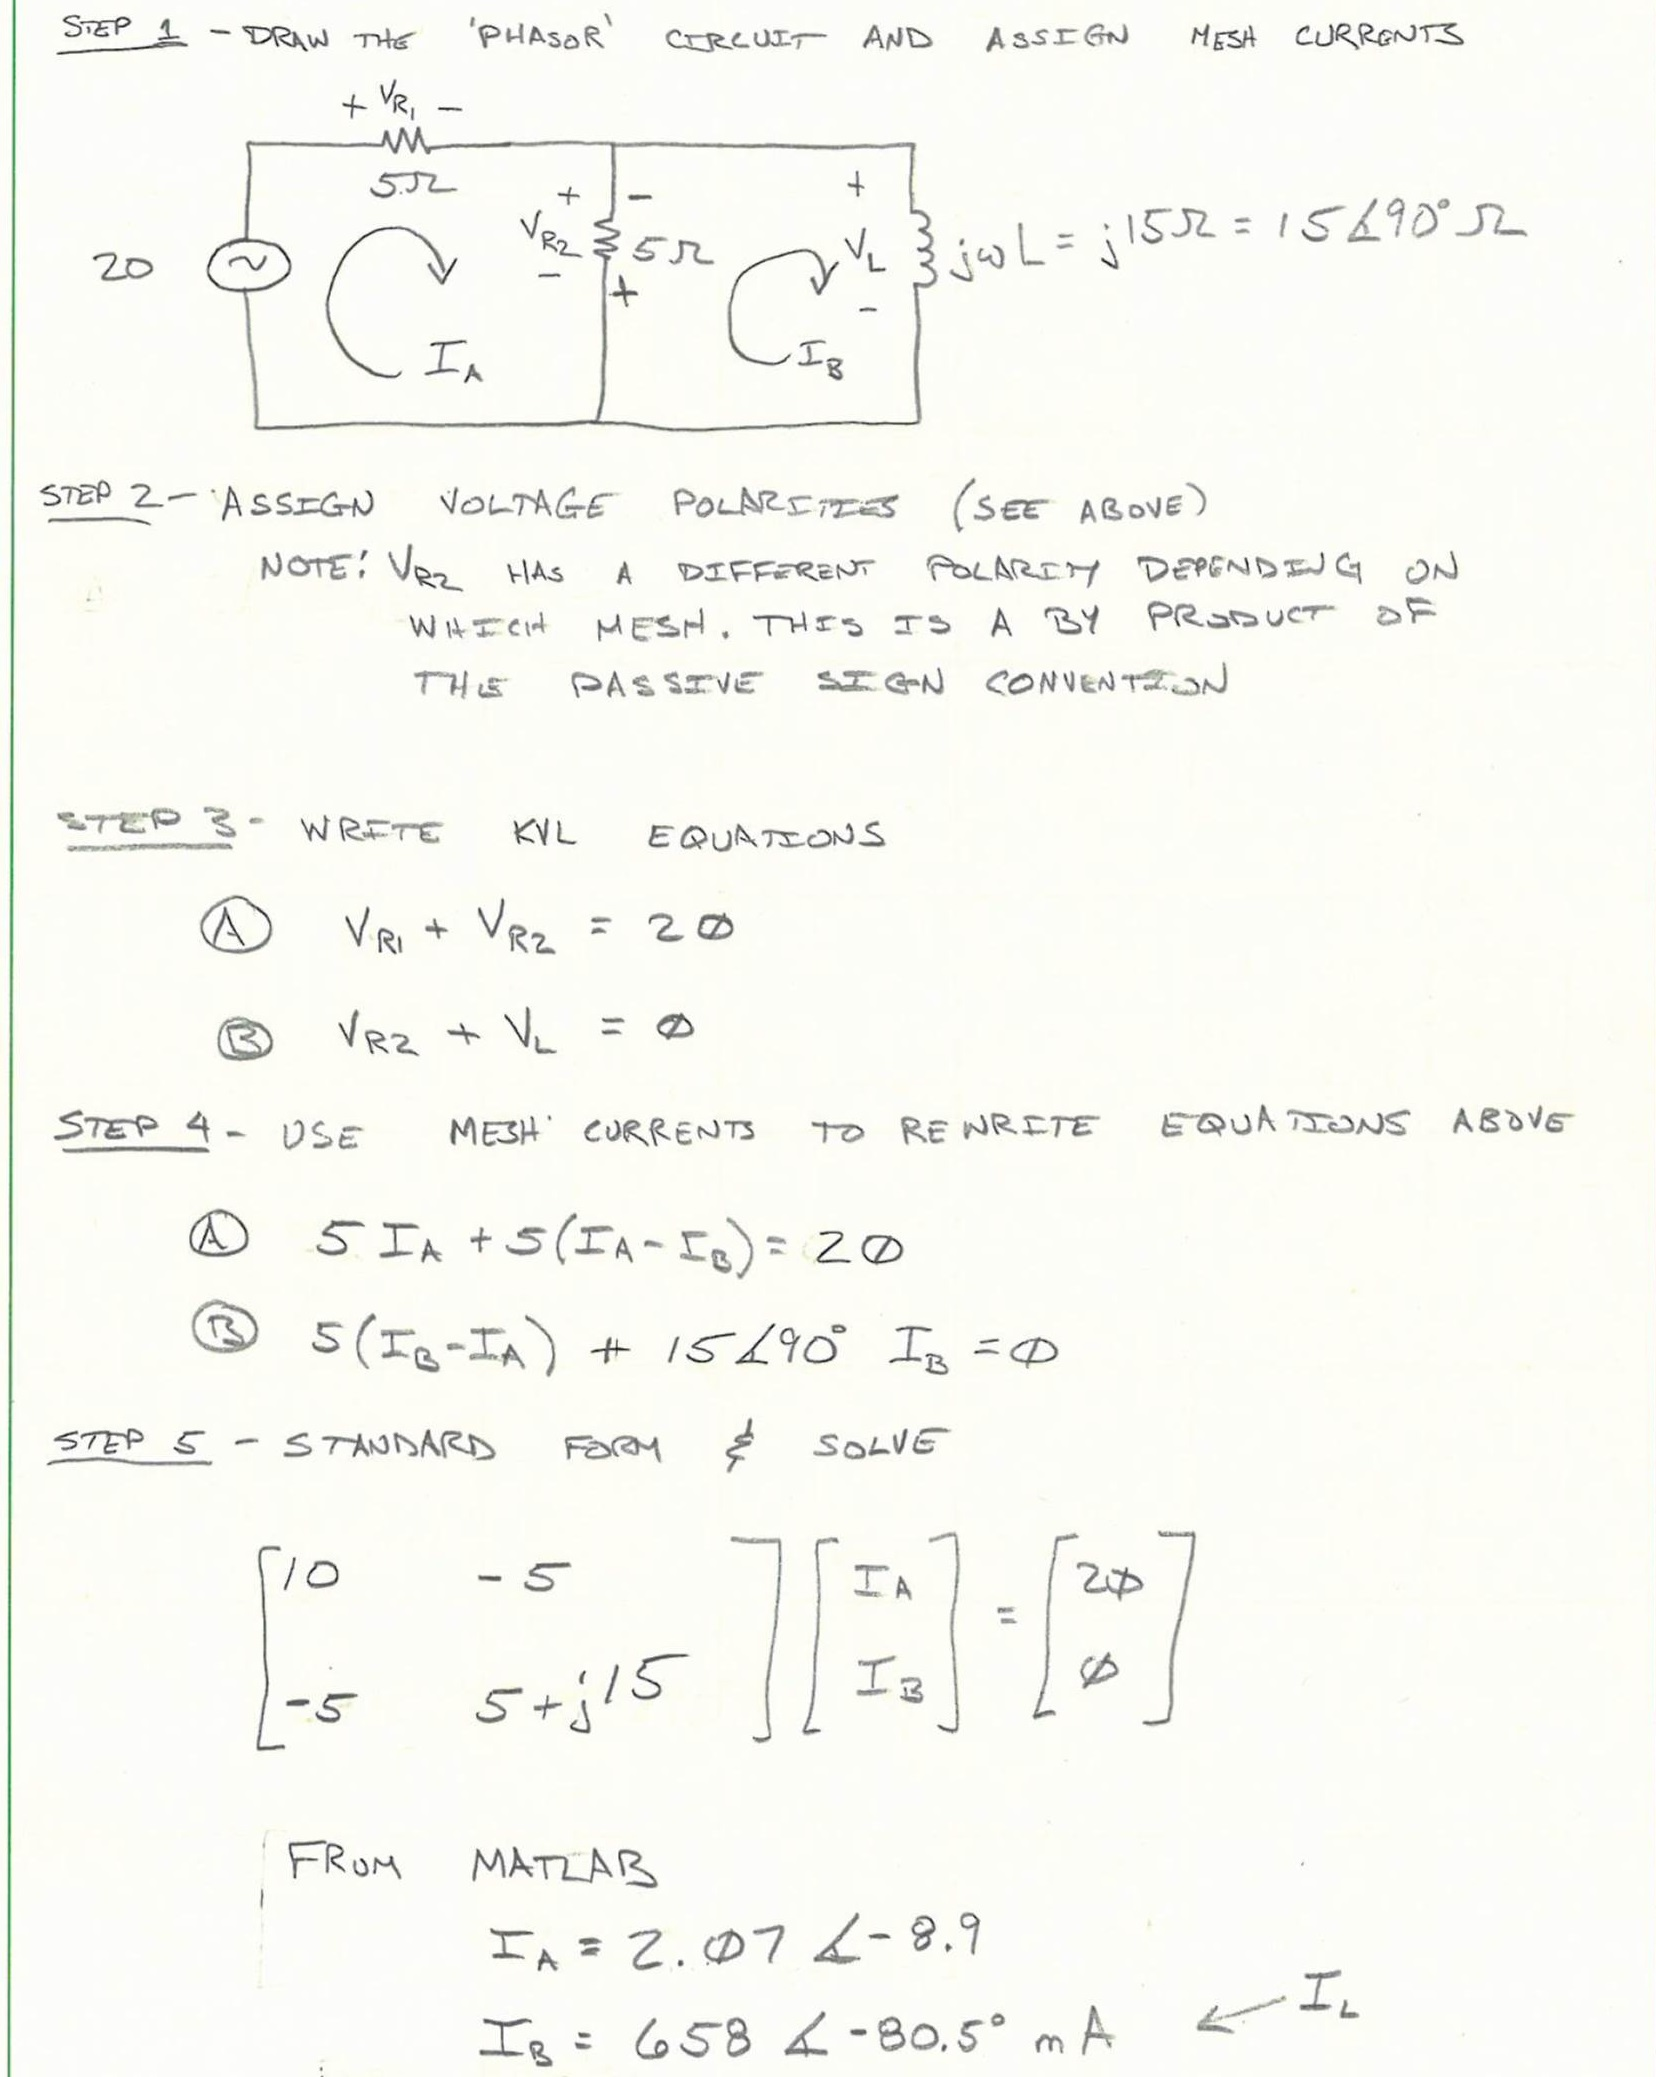
\includegraphics[width=0.65\textwidth]{Example4soln.jpg}
\end{figure}
}

\newpage
\clearpage
\pagebreak

\section{Node Voltage Analysis}
Recall the steps for Node Voltage Analysis:
\begin{enumerate}
\item Identify a \textbf{reference node}.  You will not write an equation for this node, but the voltages at the other nodes will use this as a reference.
\item Write \textbf{KCL equations} at the other $N-1$ nodes
\item Write the currents in the KCL equations in terms of \textbf{node voltages} and resistances
\item Rearrange the equations above into \textbf{standard form}
\end{enumerate}

Also recall that the steps above apply strictly to circuits with no voltage sources, but we offered three methods for dealing with voltage sources: source transformation, smart choice of a reference node, or super-nodes.

\textbf{Example 5} -- Let's rework example 3 once more, this time with Node Voltage Analysis.

\soln{6in}{
\begin{figure} [h!]
\centering
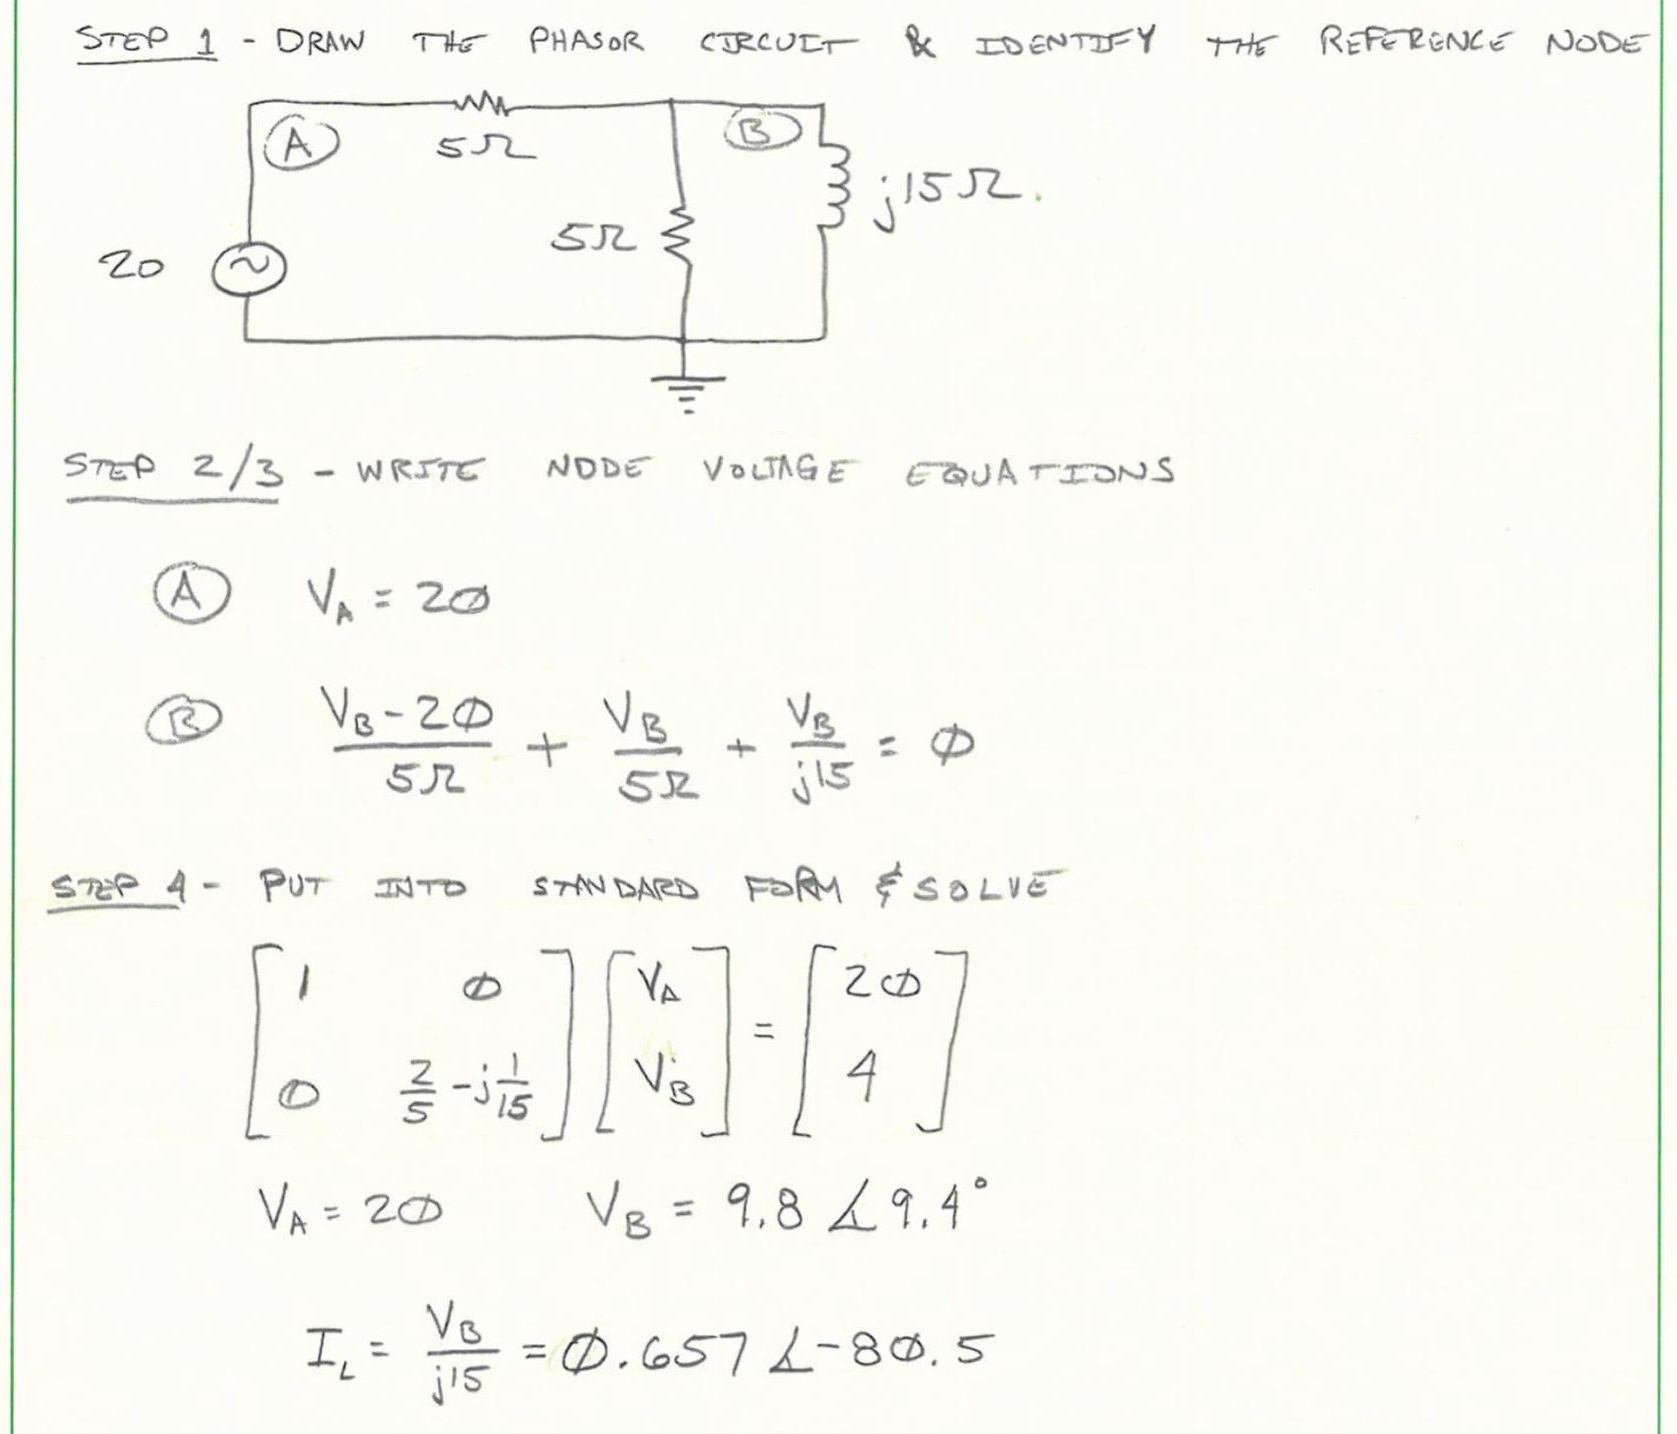
\includegraphics[width=0.95\textwidth]{Example5soln.jpg}
\end{figure}
}





\newpage
\clearpage
\pagebreak
% 
% \newpage
% \clearpage
% \pagebreak
%
% \newpage
% \clearpage
% \pagebreak
%
% \newpage
% \clearpage
% \pagebreak
%
% \newpage
% \clearpage
% \pagebreak
%
% \newpage
% \clearpage
% \pagebreak




\end{document}


% Equation Array Example Code
%\begin
%{eqnarray}
%P_R &=& i_R^2R \nonumber \\
%P_R &=& (100\ mA)^2 \times 100\ \Omega \nonumber \\
%P_R &=& (100 \times 10^{-3}\ A)^2 \times 100\ \Omega \\
%P_R &=& 10000 \times 10^{-6}\ A^2  \times 100\ \Omega \nonumber \\
%P_R &=& 1\ W  \nonumber
%\end{eqnarray}

% Figure Example Code
%\begin{figure} [h!]
%\centering
%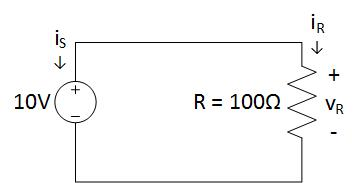
\includegraphics[width=0.5\textwidth]{OhmsLawExampleSolution.jpg}
%\caption{Ohm's Law example circuit}
%\label{fig: OhmsLawExampleSolution}
%\end{figure}

%Table Example Code
%\begin{table}[h]
%\centering
%\begin{tabular}{|l|c|c|}
%\hline
%Prefix & Abbreviation & Value \\
%\hline \hline
%Giga & $G$ & $10^9$ \\
%Mega & $M$ & $10^6$ \\
%Kilo & $k$ & $10^3$ \\
%\hline
%milli & $m$ & $10^{-3}$ \\
%micro & $\mu$ & $10^{-6}$ \\
%nano & $n$ & $10^{-9}$ \\
%pico & $p$ & $10^{-12}$ \\
%\hline
%\end{tabular}
%\caption{Engineering prefixes and values}
%\label{tab: Eng Prefixes}
%\end{table}
